\documentclass[11pt,a4paper]{article}
\usepackage[margin=2.4cm]{geometry}
\usepackage{amsmath,amssymb,amsthm,bm,mathtools}
\usepackage{booktabs}
\usepackage{graphicx}
\usepackage{tikz}
\usetikzlibrary{decorations.pathmorphing,arrows.meta,patterns}
\usepackage[most]{tcolorbox}
\usepackage[colorlinks=true,linkcolor=blue!50!black,citecolor=blue!50!black,urlcolor=blue!50!black]{hyperref}
\usepackage{enumitem}
\emergencystretch=1.5em
\usepackage{caption}
\captionsetup{font=small,labelfont=bf}

\newcommand{\kT}{k_{\mathrm B}T}
\newcommand{\dd}{\mathrm{d}}
\newcommand{\avg}[1]{\left\langle #1\right\rangle}
\newcommand{\lam}{\bm{\lambda}}
\newcommand{\Wd}{W_{\rm diss}}
\newcommand{\dFJ}{\widehat{\Delta F}_J}
\newtcolorbox{note}[1][]{colback=blue!3,colframe=blue!40!black,fonttitle=\bfseries,title=#1}

\title{Jarzynski equality for a pulled polymer in 2D\\[0.3em]
\large Model, numerical scheme and results}
\author{}
\date{6 October 2026}

\begin{document}
\maketitle

\begin{abstract}
A two-dimensional bead--spring chain is anchored at one end and pulled at the other by a
harmonic trap moving at constant speed through a Langevin heat bath. From $10^5$ independent
pulls per parameter set we measure the distribution of the work $W$ and estimate the
free-energy difference $\Delta F$ with the Jarzynski equality. Every estimate is compared
with an exact value: a closed form for the Gaussian chain, and a log-space convolution for
the stiff-bond chain. We vary the pulling time $\tau$, the temperature $T$ and the number of
beads $N$. The equality holds in all cases where enough pulls are available. What decides
whether it is usable is the dissipated work in units of $\kT$, $\beta\Wd$. This quantity is
set by friction and pulling speed, and an affine-stretching argument predicts it within
$12\%$ for $N\ge10$. At fixed $\tau/\tau_1$ it is independent of temperature but grows linearly with $N$,
so the number of pulls needed grows exponentially with chain length. Reverse pulls confirm the
Crooks fluctuation theorem, and the two-sided Bennett estimator recovers $\Delta F$ where
one-sided Jarzynski fails.

\smallskip\noindent\emph{Full derivations} (the three proofs of the Jarzynski equality, how it
determines $F$, the Crooks theorem, and the derivation of every estimator) are in the companion
\textbf{theory document} \texttt{theory.pdf}. This report summarises them and focuses on the results.
\end{abstract}

\begin{note}[Main results]
\begin{enumerate}[leftmargin=*,itemsep=2pt]
\item \textbf{Validation.} For the Gaussian chain the simulated $\avg W$ and $\mathrm{Var}\,W$
agree with the exact moments of the discrete algorithm to $0.1\%$ and $1\%$. The discrete
scheme satisfies Jarzynski to $O(\Delta t^2)$ ($8\times10^{-4}\,\kT$ at $\Delta t=0.01$).
\item \textbf{Entropic vs.\ energetic elasticity.} For the stiff-bond chain $\Delta F\propto T$
(rubber elasticity); for the Gaussian chain $\Delta F$ is independent of $T$. At fixed
$\tau/\tau_1$ the work distributions of the stiff-bond chain at different temperatures
collapse onto one curve in the variable $\beta W$.
\item \textbf{Dissipation law.} For slow enough pulls, $\beta\Wd\simeq \pi^2N/(6\,\tau/\tau_1)$:
it depends only on the reduced speed and on $N$, not on $T$. At fixed $\tau$, $\beta\Wd\propto1/T$.
\item \textbf{Convergence.} $\dFJ$ is accurate when $M\gg e^{\beta\Wd}$. In the
intermediate regime its typical error is upward, but a single rare trajectory can push it
below $\Delta F$. Bootstrap error bars become over-confident by about $3\times$.
\item \textbf{Size.} At fixed $\tau/\tau_1$ and fixed relative extension, $\beta\Wd$ grows
linearly with $N$ ($\beta\Wd=16$ at $N=40$), so the required number of pulls grows
exponentially with chain length. This is why Jarzynski is a single-molecule tool.
\item \textbf{Where the average comes from.} Plots of $e^{-\beta W}$ show that the exponential
average is carried by pulls typical of the \emph{reverse} process. For fast pulls or long chains
no forward pull reaches that region, and the estimate silently misses up to half of
$\avg{e^{-\beta W}}$.
\item \textbf{Crooks and BAR.} Reverse pulls confirm the Crooks theorem (log-ratio slope
$0.98$--$0.99$, theory $1$). Combining both directions with Bennett's acceptance ratio recovers
$\Delta F$ to within $0.01\,\kT$ at $N=40$ ($19.688\pm0.039$ vs.\ $19.694$), where forward and
reverse Jarzynski are off by $+1.47$ and $-0.76\,\kT$.
\end{enumerate}
\end{note}

\tableofcontents
\newpage

%=====================================================================
\section{Physical model}
\label{sec:model}

\begin{figure}[h]
\centering
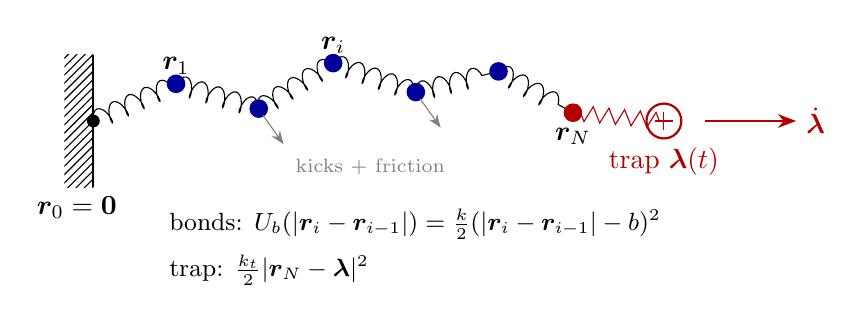
\begin{tikzpicture}[scale=1.05]
  \fill[pattern=north east lines] (-0.35,-0.8) rectangle (0,0.8);
  \draw[thick] (0,-0.8)--(0,0.8);
  \coordinate (r0) at (0,0);
  \coordinate (r1) at (1.0,0.45);
  \coordinate (r2) at (2.0,0.15);
  \coordinate (r3) at (2.9,0.7);
  \coordinate (r4) at (3.9,0.35);
  \coordinate (r5) at (4.9,0.6);
  \coordinate (r6) at (5.8,0.1);
  \foreach \a/\b in {r0/r1,r1/r2,r2/r3,r3/r4,r4/r5,r5/r6}
    \draw[decorate,decoration={coil,aspect=0.4,segment length=2.2mm,amplitude=1.2mm}] (\a)--(\b);
  \fill[black] (r0) circle (2.2pt);
  \foreach \p in {r1,r2,r3,r4,r5} \fill[blue!60!black] (\p) circle (3.2pt);
  \fill[red!70!black] (r6) circle (3.2pt);
  \node at (-0.2,-1.05) {$\bm r_0=\bm 0$};
  \node[above] at (r1) {$\bm r_1$};
  \node[above] at (r3) {$\bm r_i$};
  \node[below=2pt] at (r6) {$\bm r_N$};
  \coordinate (lam) at (6.9,0);
  \draw[red!70!black,decorate,decoration={zigzag,segment length=2mm,amplitude=1mm}] (r6)--(lam);
  \draw[red!70!black,thick] (lam) circle (6pt);
  \draw[red!70!black] (lam) +(-3pt,0)--+(3pt,0) +(0,-3pt)--+(0,3pt);
  \node[below=6pt,red!70!black] at (lam) {trap $\lam(t)$};
  \draw[-{Stealth},thick,red!70!black] (7.4,0)--(8.5,0) node[right] {$\dot{\lam}$};
  \node[anchor=west] at (0.8,-1.25) {\small bonds: $U_b(|\bm r_i-\bm r_{i-1}|)=\tfrac{k}{2}(|\bm r_i-\bm r_{i-1}|-b)^2$};
  \node[anchor=west] at (0.8,-1.8) {\small trap: $\tfrac{k_t}{2}|\bm r_N-\lam|^2$};
  \foreach \p in {r2,r4} \draw[-{Stealth},gray] (\p)++(0.05,-0.08) -- ++(0.25,-0.35);
  \node[gray] at (3.35,-0.55) {\scriptsize kicks + friction};
\end{tikzpicture}
\caption{The system. Bead $0$ is fixed at the origin. Beads $1\dots N$ move in the plane and
exchange energy with the bath. Bead $N$ is held by a harmonic trap whose centre moves from
$\lam_0$ to $\lam_1$ in a time $\tau$.}
\label{fig:schematic}
\end{figure}

The state is $\bm x=(\bm r_1,\dots,\bm r_N;\bm p_1,\dots,\bm p_N)\in\mathbb R^{4N}$, with
$\bm r_0\equiv\bm 0$. The Hamiltonian depends on the trap position $\lam\in\mathbb R^2$:
\begin{equation}
H(\bm x;\lam) = \sum_{i=1}^N \frac{|\bm p_i|^2}{2m}
 + \sum_{i=1}^N \frac{k}{2}\big(|\bm r_i-\bm r_{i-1}|-b\big)^2
 + \frac{k_t}{2}\,|\bm r_N-\lam|^2 .
\label{eq:H}
\end{equation}
$N$ is the number of mobile beads, which equals the number of bonds. The bond rest length $b$
selects one of two kinds of elasticity:
\begin{itemize}[leftmargin=*]
\item $b=0$, \textbf{Gaussian (Rouse) chain}. All forces are linear, so $\Delta F$ and even
the full work distribution are known exactly. The elasticity is \emph{energetic}: stretching
stores energy in the springs. This chain is used to validate the code.
\item $b=1$, $k b^2\gg\kT$, \textbf{nearly freely-jointed chain}. Bond lengths barely change,
so stretching works against \emph{entropy}, because a stretched chain has fewer available shapes.
This is the physics model.
\end{itemize}
Simplifications: the chain is a phantom chain (no excluded volume, so it can cross itself), it has no
bending stiffness, and the bath is free-draining (no hydrodynamic interactions between beads).

\paragraph{Protocol.} The trap moves along $x$ at constant speed,
$\lam(t)=(x_0+(x_1-x_0)t/\tau,\,0)$, from $x_0=0.2L$ to $x_1=0.7L$, where $L=Nb$ is the
contour length. For $b=0$ we use the nominal length $L=0.3N$. The chain starts in
equilibrium at $\lam_0$; at $t=\tau$ it is not in equilibrium.

\paragraph{Units and parameters.} We use $m=b=\varepsilon=1$ (time unit $\sqrt{mb^2/\varepsilon}$), bond
stiffness $k=100$, trap stiffness $k_t=10$, friction rate $\gamma=1$ (bead friction coefficient
$\zeta=m\gamma$), time step $\Delta t=0.01$, and $M=10^5$ independent pulls per parameter set. Sweeps:
$\kT\in\{0.25,0.5,1,2\}$ and $N\in\{5,10,20,40\}$.

%=====================================================================
\section{Heat bath: Langevin dynamics}
\label{sec:bath}

Each bead obeys
\begin{equation}
\dd\bm r_i=\frac{\bm p_i}{m}\dd t,\qquad
\dd\bm p_i = -\nabla_{\bm r_i}H\,\dd t - \gamma\,\bm p_i\,\dd t + \sqrt{2\gamma m\kT}\;\dd\bm B_i ,
\label{eq:langevin}
\end{equation}
with independent 2D Wiener processes $\bm B_i$. Solvent collisions enter in two forms, a
systematic drag $-\gamma\bm p$ and random kicks. Random kicks alone would heat the chain
without bound: for a free bead with noise strength $\sigma$, $\tfrac{\dd}{\dd t}\avg{p^2}=-2\gamma\avg{p^2}+\sigma^2$,
which grows linearly in time when $\gamma=0$. With friction, equipartition $\avg{p^2}=m\kT$
fixes $\sigma^2=2\gamma m\kT$. This is the fluctuation--dissipation relation. At frozen $\lam$ the
Kramers equation of \eqref{eq:langevin} has the canonical distribution
$\rho_{\rm eq}=e^{-\beta H}/Z(\lam)$ as its stationary solution, and the free energy is
$F(\lam)=-\kT\ln Z(\lam)$.

\paragraph{Slowest relaxation time.} A pull is ``fast'' or ``slow'' only relative to how quickly
the chain re-equilibrates, so every pulling time is quoted in units of $\tau_1$, the relaxation
time of the slowest collective motion of the chain (derivation in the theory document, Sec.~3.2).
It is obtained in four steps:
\begin{enumerate}[leftmargin=*,itemsep=0pt]
\item On chain scales inertia is negligible (momenta relax in $1/\gamma=1$), so beads move overdamped,
$\zeta\dot{\bm r}_i=\bm F_i+$noise.
\item Each bond is replaced by a linear spring $\kappa$: $\kappa=k$ for $b=0$. For $b=1$ the bonds do not
stretch, but by the central limit theorem a chain segment has a Gaussian end-to-end distribution, i.e.\
it acts as an \emph{entropic} spring with $\kappa=2\kT/\avg{u^2}\approx1.94$ per bond in 2D.
\item The linear chain (bead $0$ fixed, trap $k_t$ on bead $N$) has stiffness matrix $K$, and each normal
mode relaxes as $e^{-\lambda_pt/\zeta}$. The slowest gives $\tau_1=\zeta/\lambda_{\min}(K)$, computed numerically.
\item Since $k_t=10\gg\kappa$, the trap almost clamps the far end. The slowest mode is then the half-wave
$\sin(\pi i/N)$ of a string fixed at both ends, with $\lambda_{\min}\simeq\kappa\pi^2/N^2$, and
\end{enumerate}
\begin{equation}
\tau_1\simeq\frac{\zeta N^2\avg{u^2}}{2\pi^2\kT}\qquad(b=1).
\label{eq:tau1}
\end{equation}
($5.22$ for $N=10$, against the exact eigenvalue $5.46$). $\tau_1\propto N^2$ is the Rouse scaling:
a disturbance must diffuse along the whole chain. $\tau_1\propto1/T$ for the entropic chain, because the entropic
spring stiffens with temperature. \emph{Correction to the theory draft:} the draft assumed a free far end, i.e.\ a quarter-wave
mode, which overestimates $\tau_1$ by a factor $4$. We use the numerically computed
eigenvalue throughout: $\tau_1=1.45,\,5.46,\,21.3,\,84.3$ for $N=5,10,20,40$ at $\kT=1$.
Since $\tau_1\propto1/T$, $\tau_1=20.8$ at $\kT=0.25$ and $2.91$ at $\kT=2$ ($N=10$). For
the Gaussian chain, $\tau_1=0.26$ ($N=10$), independent of $T$.

%=====================================================================
\section{Stochastic thermodynamics and the Jarzynski equality}
\label{sec:thermo}

\emph{This section summarises the theory. Step-by-step derivations are in the theory document
(\texttt{theory.pdf}): Sec.~4 (free energy and reversible work), Sec.~5 (three proofs of the
Jarzynski equality), Sec.~6 (what the equality says about $F$), Sec.~7 (Crooks) and Sec.~8 (estimators).}

\paragraph{Work.} The work done by the puller along one trajectory is
\begin{equation}
W=\int_0^\tau\frac{\partial H}{\partial\lam}\cdot\dot\lam\,\dd t
=-k_t\int_0^\tau(\bm r_N-\lam)\cdot\dot\lam\,\dd t ,
\end{equation}
and the heat absorbed from the bath is $Q=\Delta H-W$. The second law gives
$\avg W\ge\Delta F$, and $\Wd=\avg W-\Delta F$ is the dissipated work.

\paragraph{Jarzynski equality.} If the chain starts in equilibrium at $\lam_0$ and the dynamics at every frozen $\lam$ preserves $\rho_{\rm eq}(\cdot;\lam)$, then for any protocol
\begin{equation}
\avg{e^{-\beta W}}=e^{-\beta\Delta F}.
\label{eq:JE}
\end{equation}

\paragraph{Discrete-time proof, which is what the code implements.} Split the protocol into
steps $\lam_0,\dots,\lam_K$ and alternate two moves. First a \emph{switch} $\lam_k\to\lam_{k+1}$ at frozen
$\bm x$, which costs $\delta W_k=H(\bm x_k;\lam_{k+1})-H(\bm x_k;\lam_k)$. Then a \emph{relax} move $\bm x_k\to\bm x_{k+1}$ by
a Markov kernel $P_{k+1}$ that preserves $\rho_{\rm eq}(\cdot;\lam_{k+1})$. Define
$f_k(\bm y)=\avg{\delta(\bm x_k-\bm y)e^{-\beta W_k}}$. Then $f_0=e^{-\beta H(\cdot;\lam_0)}/Z_0$ and
\begin{equation}
f_{k+1}(\bm y)=\int f_k(\bm x)\,e^{-\beta\delta W_k}P_{k+1}(\bm x\to\bm y)\,\dd\bm x
=\frac1{Z_0}\int e^{-\beta H(\bm x;\lam_{k+1})}P_{k+1}(\bm x\to\bm y)\,\dd\bm x
=\frac{e^{-\beta H(\bm y;\lam_{k+1})}}{Z_0},
\end{equation}
so $\avg{e^{-\beta W}}=\int f_K=Z_K/Z_0$. The kinetic energy does not depend on $\lam$ and
drops out of $\Delta F$. Any discretised Langevin step preserves $\rho_{\rm eq}$ only
approximately, so the equality holds up to the integrator's invariant-measure error (Sec.~\ref{sec:dt}).

\paragraph{Cumulants.} Expanding in cumulants,
$\Delta F=\avg W-\tfrac{\beta}{2}\sigma_W^2+\tfrac{\beta^2}{6}\kappa_3-\dots$. When $W$ is
Gaussian (exactly true for $b=0$, where $W$ is a linear functional of a Gaussian process),
$\Wd=\beta\sigma_W^2/2$. Near equilibrium the same relation $\sigma_W^2\simeq2\kT\Wd$ holds
for any system (linear response).

\paragraph{From the equality to $F$.} Taking the logarithm, $\Delta F=-\kT\ln\avg{e^{-\beta W}}$:
nonequilibrium work measurements give an \emph{equilibrium} free-energy difference. Only differences
of $F$ are accessible, and in the quasi-static limit $W\to\Delta F$ because
$\partial_{\lam}F=\avg{\partial_{\lam}H}_{\lam}$. Jensen's inequality gives the second law, and
$\Pr(W<\Delta F-\zeta)\le e^{-\beta\zeta}$: the pulls that dominate the average are exponentially rare.

\paragraph{Crooks theorem and two-sided estimators.} With $P_R$ the work distribution of the reversed
protocol ($\lam_1\to\lam_0$, started in equilibrium at $\lam_1$),
\begin{equation}
\frac{P_F(W)}{P_R(-W)}=e^{\beta(W-\Delta F)},\qquad\text{equivalently}\qquad
\frac{e^{-\beta W}P_F(W)}{\avg{e^{-\beta W}}_F}=P_R(-W).
\label{eq:crooks}
\end{equation}
The second form says that the share of the exponential average contributed by forward works near
$W$ \emph{is} the mirrored reverse distribution. Bennett's acceptance ratio (BAR) solves
$\sum_F\mathrm f(\beta(W_m-\widehat{\Delta F})+\ln\tfrac{M}{M_R})=\sum_R\mathrm f(\beta(W^R_m+\widehat{\Delta F})-\ln\tfrac{M}{M_R})$,
$\mathrm f(x)=1/(1+e^x)$. It is the minimum-variance (and maximum-likelihood) way to combine forward and reverse pulls.

\paragraph{How many pulls are needed.} The estimator
$\dFJ=-\kT\ln\big(M^{-1}\sum_m e^{-\beta W_m}\big)$ is dominated by rare pulls with
$W<\Delta F$. By \eqref{eq:crooks}, these are the pulls typical of the reverse process, near
$W\approx\Delta F-\Wd^R$, and they have probability $\sim e^{-\beta\Wd^R}$ under $P_F$. This gives
Jarzynski's (2006) criterion $M\gtrsim e^{\beta\Wd^R}$, which is $e^{\beta\Wd}$ for Gaussian work. Below it
$\dFJ$ is biased towards $\avg W$. A stricter
criterion follows from the relative variance of the weights $e^{-\beta W}$, which equals
$e^{2\beta\Wd}-1$ for Gaussian work: the statistical error drops below $\kT$ only when
$M\gtrsim e^{2\beta\Wd}$. We report the effective sample size
$M_{\rm eff}=(\sum w_m)^2/\sum w_m^2$ with $w_m=e^{-\beta W_m}$.

%=====================================================================
\section{Exact free-energy references}
\label{sec:exact}

The kinetic energy cancels. In bond variables $\bm u_i=\bm r_i-\bm r_{i-1}$ (unit Jacobian,
$\bm r_N=\sum\bm u_i$) the bonds are independent, and
\begin{equation}
Z(\lam)\propto\big(g^{*N}*w\big)(\lam),\qquad g(\bm u)=e^{-\beta k(|\bm u|-b)^2/2},\quad
w(\bm s)=e^{-\beta k_t|\bm s|^2/2},
\label{eq:Zconv}
\end{equation}
i.e.\ the trap acts as an $(N{+}1)$-th bond with zero rest length.

\paragraph{Gaussian chain.} Variances add (springs in series):
\begin{equation}
\Delta F=\tfrac{1}{2}k_{\rm eff}\big(x_1^2-x_0^2\big),\qquad 1/k_{\rm eff}=N/k+1/k_t ,
\label{eq:dFA}
\end{equation}
which is independent of $T$. For $N=10$: $\Delta F=10.125$.

\paragraph{Stiff-bond chain.} Keeping only the second moment of each bond gives the
\emph{entropic-spring} approximation
$\Delta F\approx\kT(x_1^2-x_0^2)/(N\avg{u^2}+2\kT/k_t)$, which is proportional to $T$. The exact value comes from
iterating the radial 2D convolution in log space,
\begin{equation}
\ln h_{n+1}(R)=\ln\!\int r\,\dd r\,\dd\theta\;g(r)\,h_n\!\big(\sqrt{R^2+r^2-2Rr\cos\theta}\big),
\end{equation}
with log-sum-exp quadrature ($\Delta R=0.01$, 161 radial and 256 angular nodes). The Fourier
(Hankel) route $\int\hat g(q)^N\hat w(q)J_0(q\lambda)q\,\dd q$ is mathematically equivalent
but cancels catastrophically when $Z(\lam_1)/Z(\lam_0)\lesssim10^{-4}$; it even returned negative
values at $N=40$. The log-space method reproduces Eq.~\eqref{eq:dFA} to $10^{-4}$ (at $N=40$:
$64.796$ vs.\ $64.800$) and agrees with the Hankel route to $<10^{-3}$ wherever that route is
reliable (tested for $N=3,12$).

\begin{table}[h]
\centering\small
\begin{tabular}{lccccc}
\toprule
$N$, $\kT$ & exact $\Delta F$ & entropic spring & error & $\Delta F/\kT$\\
\midrule
$5$, $1$ & $1.985$ & $2.103$ & $+6\%$ & $1.98$\\
$10$, $1$ & $4.420$ & $4.286$ & $-3\%$ & $4.42$\\
$20$, $1$ & $9.491$ & $8.654$ & $-9\%$ & $9.49$\\
$40$, $1$ & $19.694$ & $17.391$ & $-12\%$ & $19.69$\\
\midrule
$10$, $0.25$ & $1.156$ & $1.111$ & $-4\%$ & $4.62$\\
$10$, $0.5$ & $2.276$ & $2.195$ & $-4\%$ & $4.55$\\
$10$, $2$ & $8.365$ & $8.182$ & $-2\%$ & $4.18$\\
\bottomrule
\end{tabular}
\caption{Exact $\Delta F$ for the stiff-bond chain ($b=1$, protocol $0.2L\to0.7L$).}
\label{tab:dF}
\end{table}

\paragraph{What the table shows.}
(i) $\Delta F/\kT$ is almost independent of $T$: elasticity is entropic. The small
drift ($4.62\to4.18$) comes from bond stretching, which makes $\avg{u^2}$ grow from $1.008$ to
$1.06$ as $T$ rises. (ii) At fixed relative extension $\Delta F$ is nearly
\emph{extensive}: $0.40$, $0.44$, $0.47$, $0.49\,\kT$ per bead for $N=5,10,20,40$. (iii) The entropic spring underestimates $\Delta F$ for long chains (finite
extensibility at $70\%$ stretch). It \emph{overestimates} it for $N=5$, because short 2D chains
are strongly non-Gaussian. A 3-bond chain even has its end-to-end density peaked near $R\approx b$ rather
than at $R=0$. The approximation's error decays like $1/N$ at small extension (unit test).

%=====================================================================
\section{Numerical scheme}
\label{sec:numerics}

\paragraph{Integrator (BAOAB).} The Langevin generator is split into kick (B), drift (A) and
Ornstein--Uhlenbeck (O) parts, each solved exactly and applied in the order B--A--O--A--B:
\begin{align*}
\text{B}:&\ \bm p\leftarrow\bm p+\tfrac{\Delta t}{2}\bm F(\bm r;\lam),\qquad
\text{A}:\ \bm r\leftarrow\bm r+\tfrac{\Delta t}{2m}\bm p,\\
\text{O}:&\ \bm p\leftarrow e^{-\gamma\Delta t}\bm p+\sqrt{(1-e^{-2\gamma\Delta t})m\kT}\,\bm\xi,
\quad \bm\xi\sim\mathcal N(0,\mathbb 1).
\end{align*}
The O step satisfies fluctuation--dissipation exactly for any $\Delta t$. BAOAB has the
smallest configurational bias among standard splittings (Leimkuhler \& Matthews 2013) and needs
one force evaluation per step. The fastest mode is the bond stretch, $\omega_{\max}\approx2\sqrt{k/m}=20$;
with $\Delta t=0.01$, $\omega_{\max}\Delta t=0.2$.

\paragraph{Work bookkeeping.} At every step: (1) $W\mathrel{+}=\tfrac{k_t}{2}[(x_N-\lambda_{k+1})^2-(x_N-\lambda_k)^2]$
at the current $x_N$; (2) one BAOAB step at $\lam_{k+1}$. This is literally the
switch/relax scheme of the proof. A unit test checks $\Delta H=W+Q$ per trajectory to $10^{-9}$.

\paragraph{Exact initial ensemble (tilted rejection sampling).} Every pull must start from the
equilibrium ensemble at its initial trap position. Instead of equilibrating each chain dynamically,
we draw exact equilibrium configurations (theory document, Sec.~10.2):
\begin{enumerate}[leftmargin=*,itemsep=0pt]
\item \emph{Target.} In bond variables the Boltzmann weight is $\prod_ig(\bm u_i)\times w(\lam-\bm R)$,
$\bm R=\sum_i\bm u_i$. The bonds would be independent if it were not for the trap factor $w$, which only depends on the end point.
\item \emph{Plain rejection.} Draw a free chain (independent bonds) and keep it with probability
$w(\lam-\bm R)\le1$, the trap's Boltzmann factor. Kept chains are exact samples, but a free chain
rarely ends where a stretched one should. For the reverse pulls at $N=40$ ($\lambda=28$, while free chains end at
$|\bm R|\sim6$) only $\sim10^{-9}$ of the proposals are kept.
\item \emph{Tilt.} Draw instead chains pulled by a constant force $f$ along $x$, density
$\prod_ig(\bm u_i)e^{\beta fu_{i,x}}$. The bonds remain independent and easy to draw (length by inverse
CDF of $r\,g(r)I_0(\beta fr)$, angle from a von Mises law), and the proposed chains are already stretched.
\item \emph{Correction.} The ratio target/proposal is $w(\lam-\bm R)e^{-\beta fR_x}\propto e^{-\beta k_t|\bm R-\lam'|^2/2}\le1$ with
$\lam'=\lam-(f/k_t)\hat{\bm x}$, so the chain is kept with that probability. This is exact for any $f$;
$f$ only changes the efficiency.
\item \emph{Choice of $f$.} $f$ is set to the chain tension at that extension (proposal mean end
$=\lam'$). The acceptance rate rises to about $1\%$ at $N=40$ and $2$--$3\%$ at $N=10$.
\end{enumerate}
There is thus no equilibration run and no equilibration error. The forward runs of the first version used $f=0$, which
samples the same distribution exactly but more slowly.

\paragraph{Implementation and cost.} The code is in Python. Sampling is done in NumPy; the integrator runs in PyTorch (float64) on the
GPU (RTX 2060), vectorised over the $M$ independent replicas, with a cost of about 2--15\,ms per step for
$M=10^5$. The largest run ($N=40$, $3.4\times10^4$ steps, $10^5$ chains) took $16$ minutes including sampling. All runs are cached in
\texttt{data/runs/}.

\paragraph{Estimators.} For each parameter set we report $\avg W$, $\sigma_W$, $\dFJ$, the
second-cumulant estimate $\avg W-\beta\sigma_W^2/2$ and $M_{\rm eff}$. Error bars are bootstraps
over pulls (but see Sec.~\ref{sec:bootstrap}). Convergence is shown by splitting the $10^5$
pulls into disjoint blocks of $n$ and plotting the mean and spread of $\dFJ$ over blocks.

\paragraph{Unit tests (pytest, 20 tests).} The suite checks:
\begin{itemize}[leftmargin=*,itemsep=0pt]
\item forces equal $-\nabla H$ (autograd), for both chains;
\item the sampler reproduces the exact Gaussian-chain mean and covariance (also at full stretch),
the free-bond $\avg{u^2}$, and tilted and untilted samplers agree;
\item exact Crooks relations for the Gaussian chain (equal forward/reverse variances,
$\avg W_F-\Delta F=\avg W_R+\Delta F=\beta\sigma^2/2$), and BAR/reverse estimators on synthetic Crooks pairs;
\item the sampled mean trap force equals $\partial_\lambda F$ from the exact reference;
\item the log-space reference agrees with the closed form and with the Hankel route;
\item BAOAB at a fixed trap position preserves the exact equilibrium;
\item the first law holds per trajectory;
\item the simulated work moments match the exact linear theory;
\item Jarzynski holds exactly (to $10^{-3}$) for the Gaussian chain at three pulling times;
\item the estimators behave correctly on synthetic data.
\end{itemize}

\paragraph{Exact work statistics of the discrete algorithm ($b=0$).} With linear forces,
$(\bm q,\bm p,W)$ along $x$ is a linear-Gaussian Markov chain: each sub-step (switch, B, A, O)
is an affine map plus Gaussian noise. Propagating the mean vector and covariance matrix
($21\times21$ for $N=10$) through all steps gives the \emph{exact} $\avg W$ and $\mathrm{Var}\,W$
of the simulated algorithm, including all $\Delta t$ effects.

\subsection{Time-step error}
\label{sec:dt}
For the Gaussian chain the exact linear propagation gives the residual
$\avg W-\beta\sigma_W^2/2-\Delta F$ directly. It is $-8.0\times10^{-4}$, $-3.0\times10^{-3}$ and $-1.1\times10^{-2}\,\kT$ at
$\Delta t=0.01,0.02,0.04$ ($\tau=0.2$), a clean $O(\Delta t^2)$ law. The residual is not zero, although BAOAB
samples harmonic configurations exactly, because the scheme's \emph{momentum} distribution is
slightly distorted while the proof requires the full phase-space measure to be preserved. For the
stiff-bond chain ($N=10$, $\tau=4\tau_1$, $10^5$ pulls per run), halving $\Delta t$ from
$0.01$ to $0.005$ changed the three-seed mean of $\beta\dFJ$ by $-0.07$ ($\kT=2$) and $-0.05$
($\kT=1$). This is comparable to the seed-to-seed scatter of single estimates ($0.05$--$0.07$),
and $\avg W$ changed by less than $0.1\%$. No time-step effect is detectable. The time step is therefore not a limitation at the accuracy
reached here.

%=====================================================================
\section{Results}
\label{sec:results}

\subsection{Validation on the Gaussian chain (F1)}

\begin{figure}[h]
\centering
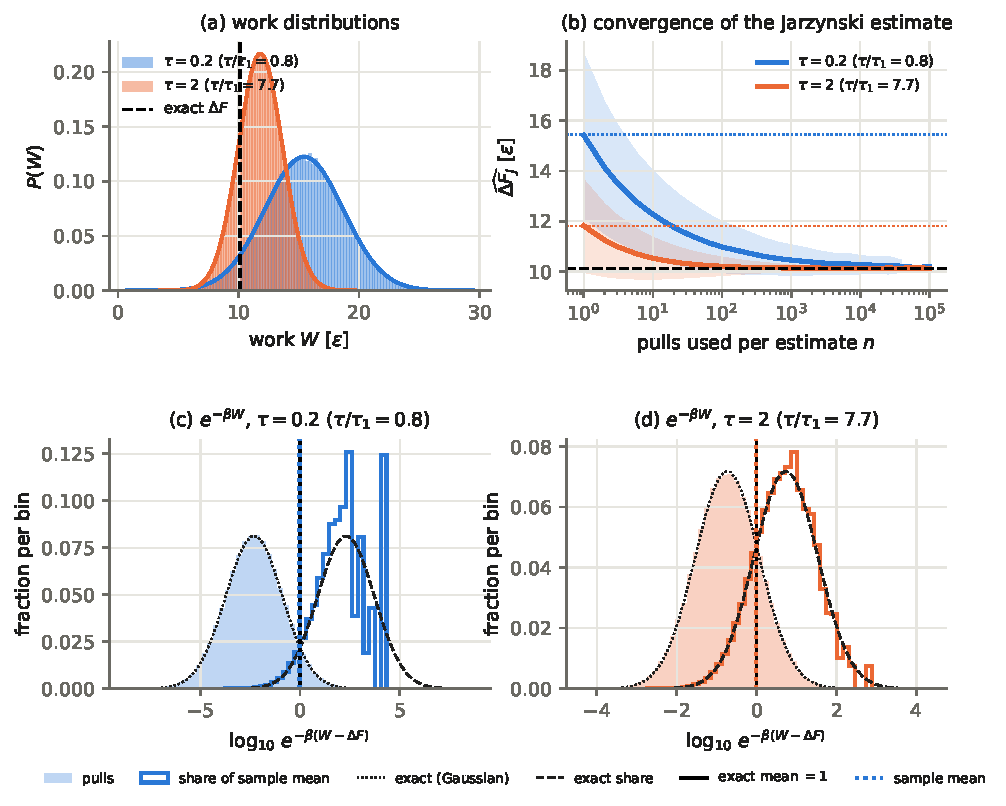
\includegraphics[width=\linewidth]{../figures/F1_validation.pdf}
\caption{Gaussian chain, $N=10$, $\kT=1$, $10^5$ pulls per speed.
(a) Simulated work histograms; lines are the exact Gaussian distribution with moments
from the linear propagation; dashed line: exact $\Delta F=10.125$.
(b) Jarzynski estimate using $n$ pulls: mean (line) and $\pm1$ s.d.\ (band) over disjoint
blocks; dotted lines: $\avg W$.
(c, d) Distribution of the Jarzynski weight $x=e^{-\beta W}/e^{-\beta\Delta F}$ (log scale), whose exact
mean is $1$. Filled: fraction of pulls; solid step: share of the sample mean contributed by each
bin ($x\times$count$/\sum x$); dashed: exact share (Gaussian theory); dotted: exact distribution of pulls;
vertical lines: exact mean $1$ (black) and sample mean (coloured, dotted).}
\label{fig:F1}
\end{figure}

\begin{center}\small
\begin{tabular}{lcccccc}
\toprule
$\tau$ ($\tau/\tau_1$) & exact $\Delta F$ & $\avg W$ sim / exact & $\sigma_W^2$ sim / exact & $\beta\Wd$ & $\dFJ$ & $M_{\rm eff}$\\
\midrule
$0.2$ ($0.8$) & $10.125$ & $15.420$ / $15.435$ & $10.64$ / $10.62$ & $5.30$ & $10.19\pm0.14$ & $51$\\
$2$ ($7.7$) & $10.125$ & $11.816$ / $11.816$ & $3.41$ / $3.38$ & $1.69$ & $10.134\pm0.015$ & $4348$\\
\bottomrule
\end{tabular}
\end{center}

\noindent\textbf{Reading.} Simulation and exact theory agree within statistical error, both for
the moments and for the whole distribution (Fig.~\ref{fig:F1}a). $\dFJ$ recovers
$\Delta F=10.125$ for both speeds, even though the average work overshoots it by
$5.3\,\kT$ for the fast pull. Panel (b) shows the characteristic finite-sample behaviour: with a
handful of pulls the estimate sits near $\avg W$, and it converges only once $n$ exceeds a
few hundred to a few thousand pulls. The faster pull needs about $100\times$ more pulls,
consistent with the $e^{\beta\Wd}$ to $e^{2\beta\Wd}$ scaling.

\noindent\textbf{Where the exponential average comes from} (panels c, d). The weight
$x=e^{-\beta(W-\Delta F)}$ has mean exactly $1$, but its distribution is extremely skewed. Most pulls
have $x\ll1$ (they dissipate), and the mean is carried by a few pulls with $x\gg1$. The contribution
to the mean (``share'') is shifted relative to where the pulls are, by $\beta^2\sigma_W^2/\ln 10$
decades for Gaussian work. For the slow pull (d) the shift is $1.5$ decades, the two
histograms overlap strongly, and the sampled share follows the exact one. For the fast pull (c) the
shift is $4.6$ decades. The exact share peaks at $x\approx10^{2.3}$, which only $0.06\%$ of pulls reach (about $60$ of $10^5$), and
extends to $x\sim10^{7}$. The sampled share is a handful of spikes that stops near $x\approx10^{4}$, so
the sample mean rests on a few dozen pulls ($M_{\rm eff}=51$). That it still lands within
$0.07\,\kT$ of the truth is helped by the Gaussian tail decaying fast.

\subsection{Effect of the pulling speed (F2)}

\begin{figure}[h]
\centering
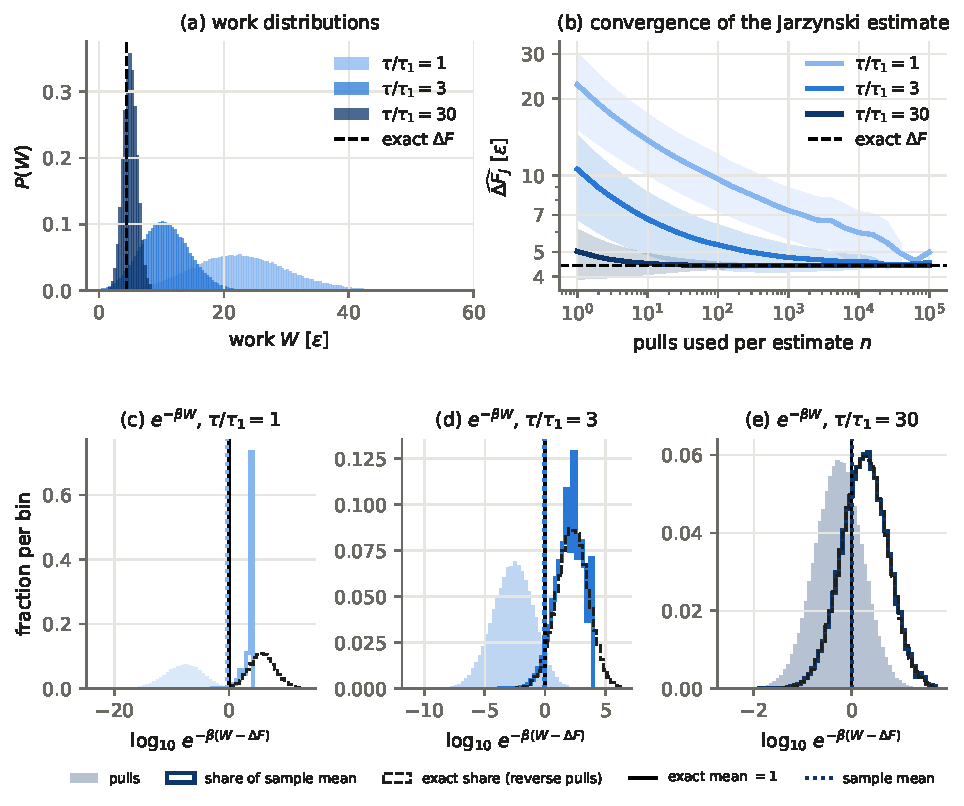
\includegraphics[width=\linewidth]{../figures/F2_speed.pdf}
\caption{Stiff-bond chain, $N=10$, $\kT=1$, $\tau_1=5.46$, $10^5$ pulls per speed.
(a) Work distributions; dashed: exact $\Delta F=4.420$. (b) Block-averaged Jarzynski estimate
using $n$ pulls (line: mean over blocks, band: $\pm1$ s.d.).
(c--e) Distribution of $x=e^{-\beta(W-\Delta F)}$ as in Fig.~\ref{fig:F1}. Here the exact share of the
mean (dashed) comes from $10^5$ \emph{reverse} pulls through Crooks' identity \eqref{eq:crooks}.}
\label{fig:F2}
\end{figure}

\begin{center}\small\setlength{\tabcolsep}{4pt}
\begin{tabular}{lccccccccc}
\toprule
$\tau/\tau_1$ & exact $\Delta F$ & $\avg W$ & $\sigma_W$ & skew & $\beta\Wd$ & affine est. & $\dFJ$ & $\avg W-\tfrac{\beta}{2}\sigma_W^2$ & $M_{\rm eff}$\\
\midrule
$1$ & $4.420$ & $22.71$ & $7.52$ & $0.21$ & $18.3$ & $16.4$ & $4.99\pm0.48$ & $-5.54$ & $4.9$\\
$3$ & $4.420$ & $10.58$ & $3.86$ & $0.16$ & $6.16$ & $5.48$ & $4.55\pm0.10$ & $3.12$ & $103$\\
$30$ & $4.420$ & $5.03$ & $1.12$ & $0.05$ & $0.61$ & $0.55$ & $4.415\pm0.005$ & $4.404$ & $30784$\\
\bottomrule
\end{tabular}
\end{center}

\noindent\textbf{Dissipation law.} In a slow pull the chain stretches affinely: bead $i$ moves
with velocity $\approx v\,i/N$, $v=(x_1-x_0)/\tau$. The friction power is then
$\sum_i\zeta(vi/N)^2\approx\zeta Nv^2/3$. With $x_1-x_0=N/2$ and Eq.~\eqref{eq:tau1},
\begin{equation}
\beta\Wd\simeq\frac{\zeta N(x_1-x_0)^2}{3\kT\tau}=\frac{\pi^2}{6}\,\frac{N}{\tau/\tau_1}.
\label{eq:affine}
\end{equation}
The simulation exceeds this estimate by $11$--$12\%$ at every speed, so the scaling
$\Wd\propto1/\tau$ holds down to $\tau=\tau_1$. The near-equilibrium relation
$\sigma_W^2=2\kT\Wd$ holds to $3\%$ at $\tau/\tau_1=30$, but fails by $\times1.2$ and $\times1.5$
for the faster pulls: the work distribution becomes broader than linear response predicts
and positively skewed. At $\tau=\tau_1$ the second-cumulant estimate is wrong by $10\,\kT$, while
$\dFJ$ is still within $0.6\,\kT$ because a handful of pulls ($M_{\rm eff}\approx5$) happened to
land near $\Delta F$. Its block-averaged curve (Fig.~\ref{fig:F2}b) has not converged at
$n=10^5$, as expected for $e^{18}\approx10^8$.

\noindent\textbf{A rare trajectory can push the estimate below $\Delta F$.} In a pilot run
with $10^4$ pulls at $\tau/\tau_1=3$, $\dFJ=2.62$, which is \emph{below} $\Delta F=4.42$, with
$M_{\rm eff}=1.9$. The estimate was dominated by one pull with $W=-6.3$, a $4.4\sigma$ event. We
traced that trajectory. The end bead started $0.76$ ahead of the trap centre (a $2.4\sigma$ thermal
fluctuation) and the chain stayed ahead of the trap for the whole pull: the bath did the
stretching and the trap was \emph{pushed}. Such pulls are rarer than a Gaussian model
suggests: in the $10^5$-pull runs at $\tau/\tau_1=1$ and $3$, only $4$ pulls fall below
$\avg W-3.5\sigma_W$, against $23$ for a Gaussian. The right tail is heavier ($65$ and $62$ pulls
above $+3.5\sigma_W$), hence the positive skew. A positive third cumulant is also why the second-cumulant
estimate falls \emph{below} $\Delta F$ in the table. The usual
statement that the Jarzynski estimate is ``biased upwards'' is true on average, but a single
under-sampled estimate can fail in either direction. With $10^5$ pulls the estimate is
$4.55\pm0.10$.

\noindent\textbf{Seeing the mean of $e^{-\beta W}$} (panels c--e). Thanks to Crooks, the reverse pulls
give the \emph{exact} shape of the share of $\avg{e^{-\beta W}}$ without any forward rare-event sampling.
\begin{itemize}[leftmargin=*,itemsep=1pt]
\item $\tau/\tau_1=30$: half of the true mean comes from $x>10^{0.27}$, a region reached by $14\%$ of
forward pulls. The sampled share matches the exact one, and no single pull carries more than $0.1\%$ of the mean.
\item $\tau/\tau_1=3$: half of the mean comes from $x>10^{2.3}$, reached by $0.07\%$ of pulls ($\approx70$).
The sampled share follows the exact one only on its lower half, and the largest pull carries $7\%$ of the mean.
\item $\tau/\tau_1=1$: half of the true mean comes from $x>10^{5.9}$, but the largest weight among all
$10^5$ pulls is $10^{4.3}$. \emph{No} pull reaches the region that dominates the average. The sample
mean is carried by three pulls ($33\%$, $27\%$, $14\%$) at the edge of the sampled range, and it equals
$e^{-\beta(4.99-4.42)}=0.57$ of the true mean, consistent with the missing upper half. The estimate
still looks deceptively good ($+0.57\,\kT$) because the logarithm compresses errors: missing half
of $\avg{e^{-\beta W}}$ costs only $\kT\ln2\approx0.7\,\kT$. Nothing in the forward sample itself reveals
that half of the average was never seen; the reverse pulls do.
\end{itemize}
\subsection{Temperature (F3)}

\begin{figure}[h]
\centering
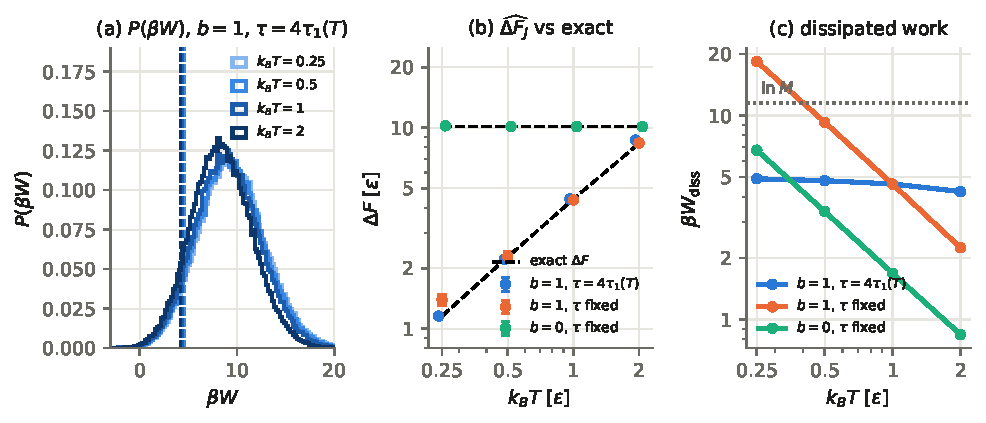
\includegraphics[width=\linewidth]{../figures/F3_temperature.pdf}
\caption{Temperature sweep, $N=10$, $10^5$ pulls per point. (a) Stiff-bond chain at fixed
reduced speed $\tau=4\tau_1(T)$: distributions of $\beta W$ (dashed: $\beta\Delta F$). (b) Jarzynski
estimates (bootstrap error bars) against the exact $\Delta F$ (dashed), for the stiff-bond chain at
fixed $\tau/\tau_1$ and at fixed $\tau=21.9=4\tau_1(\kT{=}1)$, and for the Gaussian chain at fixed
$\tau=2$. (c) $\beta\Wd$ for the same three series; dotted: $\ln M$.}
\label{fig:F3}
\end{figure}

\begin{center}\small
\begin{tabular}{l|cccc|cccc}
\toprule
& \multicolumn{4}{c|}{$b=1$, $\tau=4\tau_1(T)$} & \multicolumn{4}{c}{$b=1$, $\tau=21.9$ fixed}\\
$\kT$ & $\Delta F$ & $\dFJ$ & $\beta\Wd$ & $M_{\rm eff}$ & $\dFJ$ & $\beta\Wd$ & $M_{\rm eff}$ & $\beta(\dFJ-\Delta F)$\\
\midrule
$0.25$ & $1.156$ & $1.155\pm0.014$ & $4.90$ & $307$ & $1.39\pm0.08$ & $18.4$ & $9$ & $+0.94$\\
$0.5$ & $2.276$ & $2.214\pm0.055$ & $4.80$ & $81$ & $2.29\pm0.12$ & $9.27$ & $17$ & $+0.03$\\
$1$ & $4.420$ & $4.425\pm0.055$ & $4.61$ & $331$ & $4.37\pm0.06$ & $4.61$ & $267$ & $-0.05$\\
$2$ & $8.365$ & $8.683\pm0.082$ & $4.24$ & $648$ & $8.394\pm0.033$ & $2.25$ & $3336$ & $+0.01$\\
\bottomrule
\end{tabular}
\end{center}

\noindent\textbf{Entropic vs.\ energetic elasticity.} For the stiff-bond chain $\Delta F$ is
proportional to $T$: a hotter chain is \emph{harder} to stretch, as in rubber. For the Gaussian chain $\Delta F=10.125$ at every
temperature (Fig.~\ref{fig:F3}b), and its measured $\avg W=11.815\pm0.002$ is also
temperature-independent. In a linear system the mean response is deterministic, and the bath only
adds variance, $\sigma_W^2\propto T$; hence $\beta\Wd\propto1/T$ exactly (green line in
Fig.~\ref{fig:F3}c, matching the linear theory to $0.3\%$).

\noindent\textbf{Collapse at fixed reduced speed.} When the pulling time is scaled with the
relaxation time, $\tau=4\tau_1(T)$, the four distributions of $\beta W$ fall on top of each other
(Fig.~\ref{fig:F3}a) and $\beta\Wd\approx4.2$--$4.9$ is nearly constant. This follows from
Eq.~\eqref{eq:affine}: $\Wd\propto\zeta/\tau\propto T$ and $\Delta F\propto T$, so temperature is
just a change of energy unit for the entropic chain. The residual drift comes from the slight
bond stretching at high $T$ (Table~\ref{tab:dF}).

\noindent\textbf{At fixed pulling speed, cold baths are harder.} At fixed $\tau$, $\Wd$ is
set by friction and speed and is nearly $T$-independent, so $\beta\Wd\propto1/T$ (orange line:
$18.4,9.3,4.6,2.2$, an exact factor of $2$ per halving of $T$). At $\kT=0.25$, $\beta\Wd$ exceeds
$\ln M=11.5$ and Jarzynski fails: $\dFJ$ is too high by $0.94\,\kT$ ($20\%$). The same
pulling experiment at $\kT\ge0.5$ recovers $\Delta F$ within $0.05\,\kT$.

\subsection{Number of beads (F4)}

\begin{figure}[h]
\centering
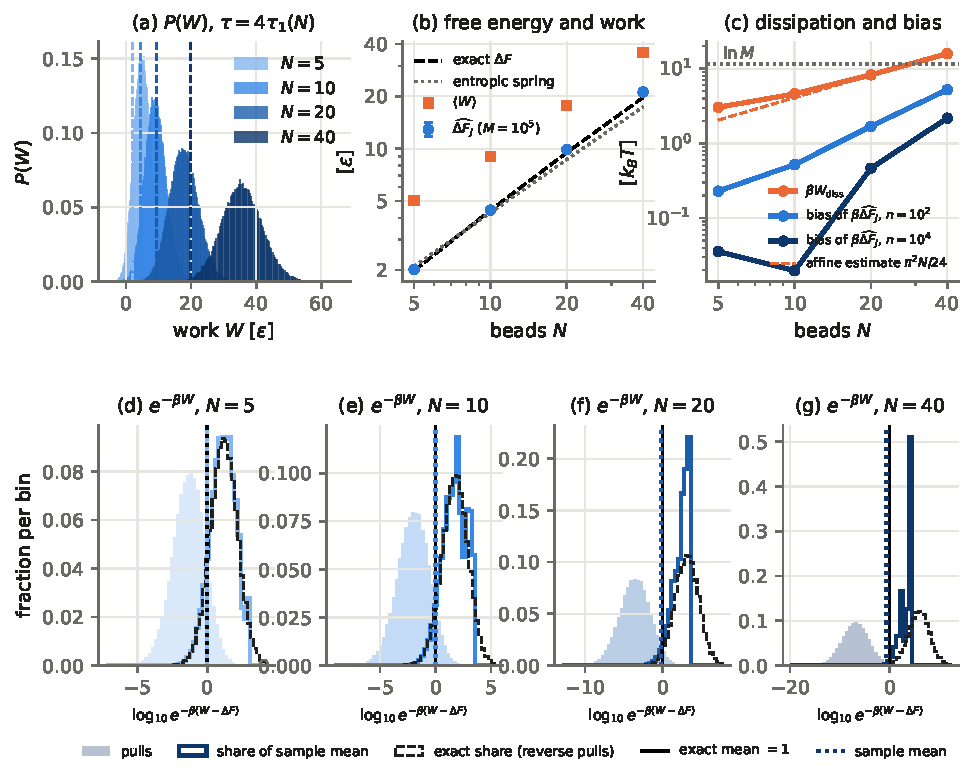
\includegraphics[width=\linewidth]{../figures/F4_size.pdf}
\caption{Stiff-bond chain, $\kT=1$, fixed relative extension $0.2L\to0.7L$, fixed reduced
speed $\tau=4\tau_1(N)$, $10^5$ pulls per point. (a) Work distributions (dashed: exact
$\Delta F$). (b) Exact $\Delta F$, entropic-spring approximation, $\avg W$ and $\dFJ$ using all
$10^5$ pulls. (c) $\beta\Wd$ and the bias of $\beta\dFJ$ when only $n$ pulls are available
(mean over disjoint blocks). (d--g) Distribution of $x=e^{-\beta(W-\Delta F)}$ for each $N$, as in
Fig.~\ref{fig:F2}; the exact share of the mean (dashed) comes from reverse pulls.}
\label{fig:F4}
\end{figure}

\begin{center}\small
\begin{tabular}{rccccccccc}
\toprule
$N$ & $\tau_1$ & $\Delta F$ & $\avg W$ & $\sigma_W$ & $\beta\Wd$ & affine \eqref{eq:affine} & $\dFJ$ ($10^5$ pulls) & $\beta(\dFJ-\Delta F)$ & $M_{\rm eff}$\\
\midrule
$5$ & $1.45$ & $1.985$ & $5.04$ & $2.64$ & $3.05$ & $2.06$ & $2.018\pm0.025$ & $+0.03$ & $1239$\\
$10$ & $5.46$ & $4.420$ & $9.03$ & $3.28$ & $4.61$ & $4.11$ & $4.429\pm0.059$ & $+0.01$ & $252$\\
$20$ & $21.3$ & $9.491$ & $17.78$ & $4.43$ & $8.29$ & $8.22$ & $9.87\pm0.11$ & $+0.38$ & $84$\\
$40$ & $84.3$ & $19.694$ & $35.65$ & $6.17$ & $15.96$ & $16.45$ & $21.16\pm0.55$ & $+1.47$ & $3.6$\\
\bottomrule
\end{tabular}
\end{center}

\noindent\textbf{Free energy and work are both extensive.} At fixed relative extension,
$\Delta F$ and $\avg W$ grow nearly linearly with $N$ (Fig.~\ref{fig:F4}b), while
$\sigma_W$ grows like $\sqrt N$ (successive ratios $1.24,1.35,1.39\to\sqrt2$). The work is a
sum of many weakly correlated contributions along the chain. Its \emph{relative} fluctuations
therefore shrink like $1/\sqrt N$, which is the approach to the macroscopic limit where
$W\to\avg W$ is sharp.

\noindent\textbf{Dissipation grows linearly with $N$ at fixed reduced speed.} $\beta\Wd=3.05,
4.61, 8.29, 15.96$ roughly doubles each time $N$ doubles. It approaches the affine estimate
$\pi^2N/24$ (within $1\%$ at $N=20$, $3\%$ at $N=40$). For $N=5$ the estimate is $1/3$ too low,
because the continuum picture of an affinely stretching chain is poor for five bonds.

\noindent\textbf{Consequence: exponential cost in system size.} The number of pulls needed,
$e^{\beta\Wd}$, is $\approx20$, $10^2$, $4\times10^3$ and $9\times10^6$ for $N=5,10,20,40$. With
$M=10^5$ the estimate is accurate up to $N=10$. It is biased by $+0.38\,\kT$ at $N=20$, where
$e^{\beta\Wd}<M<e^{2\beta\Wd}$, and fails at $N=40$ ($+1.47\,\kT$, $M_{\rm eff}=3.6$). Panel (c)
shows the bias at fixed budget: it grows steeply with $N$ for every $n$, and for $N=40$ it is
still $2.2\,\kT$ with $10^4$ pulls. The bootstrap error bars miss the exact value by $3.4\sigma$ ($N=20$) and
$2.7\sigma$ ($N=40$), the same over-confidence as in Sec.~\ref{sec:bootstrap}. Keeping
$\beta\Wd$ fixed while $N$ grows would require $\tau\propto N\tau_1\propto N^3$. This is why
Jarzynski-based free energies are a tool for single molecules and small systems.

\noindent\textbf{The breakdown seen in $e^{-\beta W}$} (panels d--g). As $N$ grows, the pull histogram
moves left (more dissipation) and the exact share of the mean moves right, so the two separate.
At $N=5$ and $10$ they overlap and the sampled share follows the exact one. At $N=20$ the sampled
share is cut off at the largest observed weight ($10^{3.5}$), and $40\%$ of the exact share lies beyond it.
At $N=40$ one pull carries $51\%$ of the sample mean and the next $13\%$, and $81\%$ of the exact share
lies beyond the largest forward weight ($10^{4.1}$). Most of the average was never sampled.

\subsection{Crooks fluctuation theorem and two-sided estimation (F5)}

For each forward run of F2 and F4 we ran $10^5$ \emph{reverse} pulls: the trap moves from $0.7L$ back
to $0.2L$ in the same time $\tau$, starting from the exact equilibrium ensemble at $0.7L$ (tilted
sampler). The reverse works $W_R$ are compared with the forward works through
Eq.~\eqref{eq:crooks}.

\begin{figure}[h]
\centering
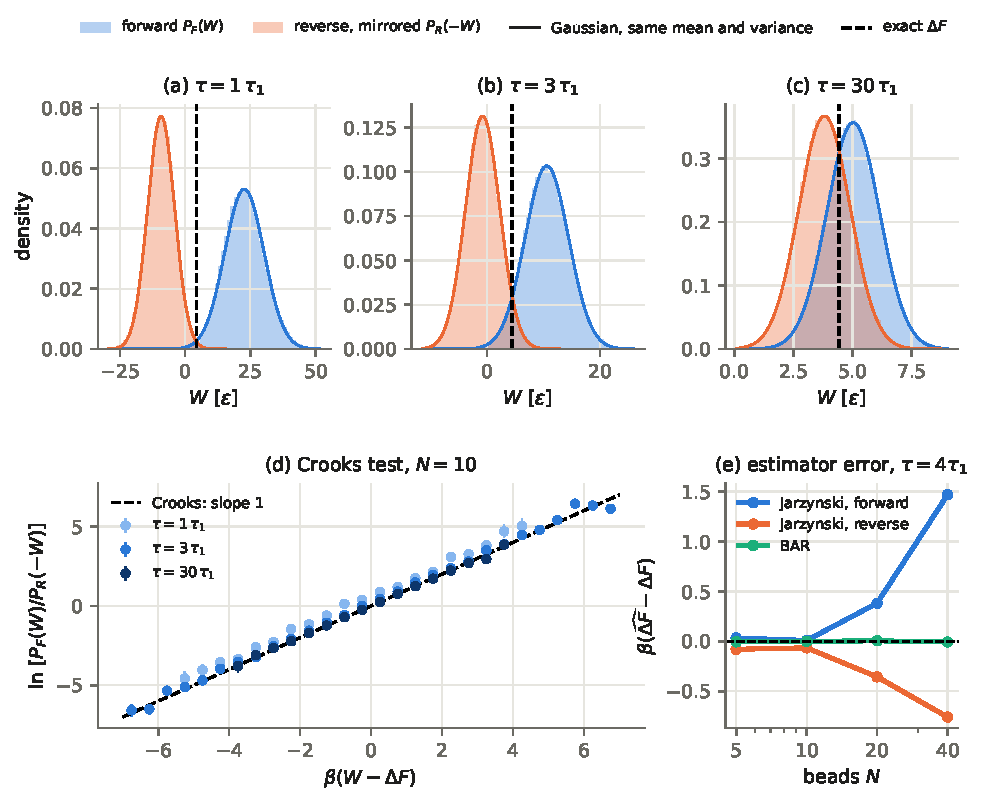
\includegraphics[width=\linewidth]{../figures/F5_crooks.pdf}
\caption{Crooks theorem, stiff-bond chain, $\kT=1$, $10^5$ forward and $10^5$ reverse pulls per point.
(a--c) $N=10$: forward work distribution $P_F(W)$ (blue) and mirrored reverse distribution $P_R(-W)$
(orange) for $\tau=\tau_1$, $3\tau_1$, $30\tau_1$. Lines are Gaussians with the same mean and variance;
the dashed line is the exact $\Delta F=4.420$, where the two distributions cross.
(d) $\ln[P_F(W)/P_R(-W)]$ against $\beta(W-\Delta F)$ in the overlap region (bins with Poisson error
$<0.5$). Crooks predicts the dashed line of slope 1 through the origin, for every speed. (e) Error of
forward Jarzynski, reverse Jarzynski and BAR against $N$ at $\tau=4\tau_1$.}
\label{fig:F5}
\end{figure}

\begin{center}\small\setlength{\tabcolsep}{4pt}
\begin{tabular}{lccccccccc}
\toprule
$\tau/\tau_1$ & exact $\Delta F$ & $\avg{W_F}$ & $\avg{W_R}$ & $\beta\Wd^F$ & $\beta\Wd^R$ & Crooks slope & $\dFJ$ fwd & $\dFJ$ rev & BAR\\
\midrule
$1$ & $4.420$ & $22.71$ & $9.21$ & $18.3$ & $13.6$ & $0.985$ & $4.99$ & $3.88$ & $4.340\pm0.039$\\
$3$ & $4.420$ & $10.58$ & $0.79$ & $6.16$ & $5.21$ & $0.994$ & $4.55$ & $4.40$ & $4.414\pm0.007$\\
$30$ & $4.420$ & $5.03$ & $-3.81$ & $0.61$ & $0.61$ & $0.983$ & $4.415$ & $4.417$ & $4.416\pm0.002$\\
\bottomrule
\end{tabular}

\smallskip
\begin{tabular}{rccccccc}
\toprule
$N$ & exact $\Delta F$ & $\beta\Wd^F$ & $\beta\Wd^R$ & $\beta(\dFJ^{\rm fwd}-\Delta F)$ & $\beta(\dFJ^{\rm rev}-\Delta F)$ & $\beta(\widehat{\Delta F}_{\rm BAR}-\Delta F)$\\
\midrule
$5$ & $1.985$ & $3.05$ & $2.76$ & $+0.033$ & $-0.080$ & $-0.005\pm0.007$\\
$10$ & $4.420$ & $4.61$ & $4.03$ & $+0.009$ & $-0.065$ & $-0.000\pm0.007$\\
$20$ & $9.491$ & $8.29$ & $7.10$ & $+0.382$ & $-0.356$ & $+0.006\pm0.013$\\
$40$ & $19.694$ & $15.96$ & $13.59$ & $+1.468$ & $-0.758$ & $-0.007\pm0.039$\\
\bottomrule
\end{tabular}
\end{center}
\noindent(BAR error bars are the spread over $10$ disjoint sub-samples divided by $\sqrt{10}$.)

\noindent\textbf{Crooks holds.} For every speed $P_F(W)$ and $P_R(-W)$ cross at $\Delta F$
(Fig.~\ref{fig:F5}a--c). The log-ratio is a straight line with slope $0.983$--$0.994$, independent
of the speed (Fig.~\ref{fig:F5}d), although the two distributions themselves change completely between
$\tau=\tau_1$ and $30\tau_1$. The residual $1$--$2\%$ is of the size expected from finite histogram bins and was
not investigated further. At $\tau=\tau_1$ the points lie slightly above the line, consistent with
the small negative BAR error below: the overlap region is thin there.

\noindent\textbf{Shapes of the forward and reverse distributions.} Both are close to Gaussian at
every speed (Fig.~\ref{fig:F5}a--c), with skewness at most $0.21$ and excess kurtosis at most $0.10$.
The reverse distribution is the \emph{narrower} one:
\begin{center}\small
\begin{tabular}{lcccccc}
\toprule
$\tau/\tau_1$ & $\sigma_F$ & $\sigma_R$ & skew$_F$ & skew$_R$ & $\sigma_F^2/2\kT\Wd^F$ & $\sigma_R^2/2\kT\Wd^R$\\
\midrule
$1$ & $7.52$ & $5.16$ & $+0.21$ & $+0.15$ & $1.54$ & $0.98$\\
$3$ & $3.86$ & $3.04$ & $+0.16$ & $-0.07$ & $1.21$ & $0.89$\\
$30$ & $1.12$ & $1.09$ & $+0.05$ & $-0.05$ & $1.03$ & $0.98$\\
\bottomrule
\end{tabular}
\end{center}
The last two columns test the linear-response relation $\sigma_W^2=2\kT\Wd$, which holds exactly for
Gaussian work near equilibrium. The reverse pull satisfies it within about $10\%$ even at $\tau=\tau_1$,
while the forward pull exceeds it by $54\%$. So the \emph{forward} pull is the more strongly
nonlinear process. A plausible reading, not tested further: in a fast forward pull the trap drags the
end into the stiff, finite-extensibility regime, where small differences in the chain's shape produce
large differences in the force and hence in the work. In a reverse pull the tension is being released
and the chain moves towards the soft, nearly Gaussian regime. Because the reverse mean work is small
($\avg{W_R}=-\Delta F+\Wd^R$, e.g.\ $0.79$ at $3\tau_1$), its spread looks large \emph{relative to its
mean}, and individual reverse works change sign. That is a cancellation between released free energy
and dissipation, not larger fluctuations. These shapes are measured from $10^5$ pulls each and are well
sampled. The sampling difficulty discussed above concerns only the far tails that dominate the
exponential averages, not the bulk of the distributions.

\noindent\textbf{Forward and reverse dissipation differ.} The reverse pull dissipates less:
$\beta\Wd^R=13.6$ vs.\ $\beta\Wd^F=18.3$ at $\tau=\tau_1$, and $13.6$ vs.\ $16.0$ at $N=40$. They become
equal only near equilibrium ($\tau=30\tau_1$), where both distributions are Gaussian and Crooks forces
$\Wd^F=\Wd^R$. A plausible reason, not tested here, is that the reverse pull starts from the stretched
chain, which is stiffer (finite extensibility) and therefore relaxes faster and keeps up with the
trap better. This asymmetry matters because, by Eq.~\eqref{eq:crooks}, forward Jarzynski needs
$M\gtrsim e^{\beta\Wd^R}$ pulls ($8\times10^5$ at $N=40$, more than we have), and reverse Jarzynski needs
$e^{\beta\Wd^F}$. The two one-sided estimators are biased in opposite directions, as expected.

\noindent\textbf{BAR fixes the size problem.} Combining both directions, BAR is within $0.01\,\kT$ of the
exact $\Delta F$ for every $N$, including $N=40$, where forward and reverse Jarzynski are off by
$+1.47$ and $-0.76\,\kT$ with the same $10^5$ pulls each. BAR needs only the \emph{overlap} of
$P_F(W)$ and $P_R(-W)$ around $\Delta F$, not the far tail of either. At $N=40$ that overlap
contains $0.4\%$ of the forward pulls (those with $W<\Delta F$) and $0.3\%$ of the reverse pulls, a few
hundred each, which is enough. At $\tau=\tau_1$ ($N=10$) the overlap is thinner and BAR is
$2\sigma$ low ($-0.08\,\kT$), still far better than either one-sided estimate ($+0.57$, $-0.54$). At
$\tau=30\tau_1$ all three estimators agree on $4.416$, $0.004\,\kT$ ($0.1\%$) below the reference, which is at
the level of the time-step error.

\subsection{Bootstrap error bars are over-confident}
\label{sec:bootstrap}
In two cases the bootstrap error bar on $\dFJ$ does not cover the exact value: the
Gaussian chain at $\kT=0.25$ ($\beta\Wd=6.8$; $+0.42\,\kT$, bootstrap $0.10\,\kT$) and the
stiff-bond chain at $\kT=2$, $\tau=4\tau_1$ ($+0.16\,\kT$, bootstrap $0.04\,\kT$). For the Gaussian
case the true sampling distribution of $\dFJ$ is computable: drawing $300$ samples of
$10^5$ Gaussian works with the exact moments gives a mean bias of $+0.10\,\kT$ and a spread of $0.28\,\kT$. The observed
$+0.42$ is therefore a $1.1\sigma$ event, but the bootstrap reports a spread $3\times$ smaller
than the truth. The bootstrap resamples only the pulls that were observed, so it cannot account
for the rare low-$W$ pulls that were never drawn. For the stiff-bond chain at $\kT=2$, three
further independent runs gave $+0.03$, $-0.06$ and $-0.00\,\kT$. The first value $+0.16\,\kT$ was
therefore a fluctuation: across the four runs the estimate scatters by $0.09\,\kT$, twice the
bootstrap error ($0.04$--$0.06\,\kT$). \emph{Practical rule:} the error bar of a single
Jarzynski estimate should come from independent repetitions (or from the block curve), not from
a bootstrap of one sample, whenever $M_{\rm eff}$ is below a few thousand.

%=====================================================================
\section{Discussion}
\label{sec:discussion}

\begin{itemize}[leftmargin=*]
\item \textbf{The equality is exact; the estimator is the bottleneck.} In every case where
$M\gg e^{\beta\Wd}$, $\dFJ$ agrees with the exact $\Delta F$, including pulls where the
average work exceeds $\Delta F$ by $6\,\kT$. In practice the whole difficulty is sampling the
left tail of $P(W)$.
\item \textbf{One dimensionless number controls everything:} $\beta\Wd\simeq(\pi^2/6)\,N/(\tau/\tau_1)$.
Temperature enters only through $\tau_1\propto1/T$. Changing $T$ at fixed $\tau$ means changing the
reduced speed, which is why cold experiments are harder.
\item \textbf{Size.} At a fixed reduced speed the dissipation is extensive in $N$, so the
number of pulls needed grows exponentially with system size. To keep $\beta\Wd$ fixed,
$\tau$ must grow like $N\tau_1\propto N^3$.
\item \textbf{Cheap diagnostics are misleading} in the dangerous regime: the second-cumulant
formula fails as soon as $P(W)$ is skewed, and the bootstrap underestimates the error by a
factor $\sim3$. $M_{\rm eff}$ and the block-convergence curve are the useful diagnostics: a
curve still drifting at the largest $n$ is unreliable.
\item \textbf{Use both directions when possible.} The exponential average is dominated by
pulls typical of the reverse process, so one-sided estimates silently miss part of it. When reverse
pulls are available, BAR needs only the overlap region and gave $\Delta F$ to $0.01\,\kT$ at $N=40$
with the same data that left one-sided Jarzynski $1.5\,\kT$ off.
\end{itemize}

\paragraph{Possible extensions (not done, suggested).}
\begin{itemize}[leftmargin=*,itemsep=1pt]
\item \emph{Lower dissipation by design}: optimise the protocol $\lambda(t)$ (not just its
duration) to minimise $\avg W$ or the variance of the estimator. In linear response the
optimum moves at constant ``thermodynamic speed''. Feedback control (a protocol that reacts to
the measured chain) can even lower $\avg W$ below $\Delta F$, at the cost of information (Sagawa--Ueda).
These are the subject of the separate optimal-protocol project. Note that the second law forbids any
open-loop protocol from shifting the whole distribution below $\Delta F$.
\item The free-energy \emph{profile} $F(\lambda(t))$ from the same pulls (Hummer--Szabo).
\item Excluded volume and bending stiffness, with $\Delta F$ from thermodynamic integration.
\end{itemize}

\begin{thebibliography}{9}
\bibitem{J97} C.~Jarzynski, Phys.\ Rev.\ Lett.\ \textbf{78}, 2690 (1997).
\bibitem{C99} G.~E.~Crooks, Phys.\ Rev.\ E \textbf{60}, 2721 (1999).
\bibitem{J06} C.~Jarzynski, \emph{Rare events and the convergence of exponentially averaged
work values}, Phys.\ Rev.\ E \textbf{73}, 046105 (2006).
\bibitem{G03} J.~Gore, F.~Ritort, C.~Bustamante, \emph{Bias and error in estimates of
equilibrium free-energy differences from nonequilibrium measurements}, PNAS \textbf{100}, 12564 (2003).
\bibitem{S98} K.~Sekimoto, Prog.\ Theor.\ Phys.\ Suppl.\ \textbf{130}, 17 (1998).
\bibitem{LM13} B.~Leimkuhler, C.~Matthews, Appl.\ Math.\ Res.\ Express \textbf{2013}, 34 (2013).
\bibitem{L02} J.~Liphardt \emph{et al.}, Science \textbf{296}, 1832 (2002).
\bibitem{Seifert} U.~Seifert, Rep.\ Prog.\ Phys.\ \textbf{75}, 126001 (2012).
\end{thebibliography}

\end{document}
